
%(BEGIN_QUESTION)
% Copyright 2013, Tony R. Kuphaldt, released under the Creative Commons Attribution License (v 1.0)
% This means you may do almost anything with this work of mine, so long as you give me proper credit

A large natural-gas fired furnace receives its fuel gas supply through a pressure regulator which drops the natural gas pressure from 30 PSI to approximately 10 inches of water column:

$$\includegraphics[width=15.5cm]{i02058x01.eps}$$

Devise a step-by-step procedure by which you may remove the pressure regulator (PCV-105) from service in order to rebuild it in the shop.  Your procedure needs to ensure that the gas pressure delivered to the furnace does not ever exceed the allowable high limit (15 "WC) or fall below the allowable low limit (8 "WC):

\begin{itemize}
\item{} 
\vskip 20pt
\item{} 
\vskip 20pt
\item{} 
\vskip 20pt
\item{} 
\vskip 20pt
\item{} 
\end{itemize}

\underbar{file i02058}
%(END_QUESTION)





%(BEGIN_ANSWER)

\begin{itemize}
\item{} Begin by slowly opening the bypass valve until either PG-16 or PG-17 begins to register a rise in pressure.  This tells you the pressure regulator PCV-105 is completely bypassed, with all natural gas passing through the hand-actuated bypass valve instead of PCV-105.
\item{} Shut the block valves in any order.
\item{} Open the bleed valve to de-pressurize the regulator.
\item{} Place safety tags on all block and bleed valves to ensure no one turns them while the pressure regulator is removed from the piping.
\item{} An operator needs to keep watch over the downstream pressure, turning the hand-actuated bypass valve as necessary to maintain proper gas pressure to the furnace.
\end{itemize}

%(END_ANSWER)





%(BEGIN_NOTES)

This question is based on an incident I faced early in my career as an instrument technician, when I almost died helping an operator place a rebuilt Fisher 1098 regulator into service.  The sequence of events went like this:

\begin{itemize}
\item{} Operators had successfully removed the regulator from service, properly bypassing and blocking the Fisher 1098 so I could remove it from the piping system.
\vskip 10pt
\item{} I took the regulator back to the shop and rebuilt it there.
\vskip 10pt
\item{} After rebuilding the regulator, I re-installed it in the piping system.  This included replacing the flange gaskets and properly re-torquing all flange bolts at the regulator flanges.
\vskip 10pt
\item{} Calling a field operator to the site, I told him that the gas pressure regulator was ready to put back into service.
\vskip 10pt
\item{} The operator begins by opening both block valves and checking for leaks at the flanges using ``Snoop'' leak detection fluid.  This fluid works much like soapy water to reveal gas leaks by producing lots of bubbles.  No leaks were detected.
\vskip 10pt
\item{} After successfully un-blocking the regulator, he begins to turn the bypass valve off.  As expected, the downstream pressure stabilizes at 10 "WC (the set regulating pressure of PCV-105) as indicated by PG-16.  The noise coming from the bypass valve diminishes, until all the flow is going through PCV-105 and none of it through the bypass valve.  Everything looks like it's operating properly.
\vskip 10pt
\item{} The operator gets a worried look on his face, saying he's concerned about the lack of noise.  As it turns out, the bypass valve had been making a lot of noise ever since the regulator had been bypassed due to the turbulence created within its butterfly design.  The Fisher 1098 regulator, by contrast, was equipped with ``whisper'' trim so that it ran very quietly doing the same throttling job.  This sudden drop in noise level was perfectly normal, but the operator mistakenly interpreted it as a lack of gas flow to the furnace, thinking the newly rebuilt regulator wasn't supplying the furnace with fuel gas.
\vskip 10pt
\item{} The field operator uses his radio to call the control room operator, asking for a report on the reading given by flow transmitter FT-83.  The control operator replies ``I read zero flow!''
\vskip 10pt
\item{} The field operator begins to panic.  I look over at the flow transmitter, and to my dismay I see that someone has removed the DP transmitter from service.  All I see where FT-83 is supposed to be is a piece of liquid-tight conduit dangling in mid-air with a single pair of wires hanging out its end.  This is the reason the control room operator is reading zero flow: {\it the transmitter isn't there!}
\vskip 10pt
\item{} Now the field operator turns his attention to pressure gauge PG-17.  It appears to be reading zero, which to him is further proof that the regulator isn't passing any fuel gas to the furnace.
\vskip 10pt
\item{} Frantic, the operator begins to open the bypass valve again, trying to re-establish (in his mind) fuel gas flow to the furnace.  Meanwhile I happen to notice that someone has installed the wrong pressure gauge for PG-17: it is a {\it 0 to 30 PSI} gauge, whereas PG-16 has the proper pressure range: {\it 0 to 30 "WC}.  The operator is looking at an incorrectly-ranged pressure gauge, thinking the pressure is far too low!
\vskip 10pt
\item{} As the operator opens the bypass valve, it begins to make its howling noise again because it is now bearing the flow of gas, the regulator having been bypassed entirely.  However, PG-17 is still reading too low (by the operator's assessment) because it's reading PSI instead of inches water column.  PG-16 is reading fine, but when I try to point this out, the operator ignores me.  
\vskip 10pt
\item{} Seeing that PG-17 is still reading too low (by his interpretation), the operator opens the bypass valve even more than before in an attempt to get that gauge to read ``10'' (PSI, not "WC).  Seeing that PG-16 is reading just fine, I try to tell him we do have fuel gas flow to the furnace, but he counters with the control room operator's report of FT-83 reading zero.  When I try to direct the operator's attention to the missing transmitter, he doesn't look.
\vskip 10pt
\item{} As the operator continues to open the hand bypass valve, three things happen: PG-17 begins to rise on its PSI scale ; PG-16's needle wraps all the way around until it comes to rest on the wrong side of the ``0'' peg ; and the bypass valve becomes quieter.  The reduction in noise is a result of the butterfly mechanism creating less turbulence as it opens wider.  The operator again makes the mistake of thinking this means {\it less} flow of gas through the system, and begins to frantically open the bypass valve further.
\vskip 10pt
\item{} Now the operator calls on his radio for another field operator to go to the furance and peer through the observation glass at the flames.  He is trying to visually verify whether or not there is still fire in the furnace.  The other field operator reports back that the view inside the furnace is completely dark.  My operator begins to ``lose it'' and opens the bypass valve even wider.
\vskip 10pt
\item{} It occurs to me that the furnace appears dark because the burners are being flooded with excess fuel gas, and thus burning terribly rich (making black smoke).  It also occurs to me that this is a very dangerous situation, as a cloud of unburnt gas inside of a hot furance could cause a violent explosion.  Bear in mind that this is a {\it huge} furnace, and it happens to be located directly overhead of where I and the operator are standing.
\vskip 10pt
\item{} I try in vain to explain to the operator that there is far too much gas being sent to the furnace, but he isn't believing me because he has these data telling him otherwise:
\itemitem{} FT-83 reads zero flow
\itemitem{} PG-17 reads too low
\itemitem{} The bypass valve is quiet
\itemitem{} The furnace shows no evidence of flame inside
\vskip 10pt
\item{} Knowing I only have moments to prevent an explosion, I consider these few options:
\itemitem{} Try rationalizing with the operator ({\it unlikely to yield different results})
\itemitem{} Physically remove the operator from the valve and take control myself ({\it would likely result in my termination from this job, and likely the end of my career as an instrument technician})
\itemitem{} Somehow convince the operator to just put everything back where it was before we started ({\it but how???})
\itemitem{} Run like hell
\vskip 10pt
\item{} Suddenly an idea occurs to me: I point to my watch and tell the operator ``Look at the time -- our shift is nearly over.  Why don't we just put everything back where we started, and try again tomorrow?''
\vskip 10pt
\item{} To my relief, this tactic works.  The operator closes the bypass valve back to where it was previously, where it begins to howl again.  ``Look, the flow's come back!'' is the operator's response.  PG-16 unwinds itself and returns to a normal pressure reading.  The other field operator reports that he now sees flame inside the furnace.
\vskip 10pt
\item{} Shaking with adrenaline, I walk back to the instrument shop.
\vskip 10pt
\item{} The next day I return to the site, armed with a replacement pressure transmitter for FT-83 and a new gauge for PG-17.  When I arrive, I am surprised to find everything's been put back into service for me.  Apparently the night shift was tired of hearing the howling of the bypass valve, and put the regulator back into service without incident.
\end{itemize}

\vskip 10pt

After relating this sequence of events to your students, you should ask them to comment on what could have been done to avoid this scenario.  There are several things that could have been done differently, both by the operators (all three of them) and by myself (the technician).

%INDEX% Final Control Elements, gas pressure regulator: (GRAPHIC ILLUSTRATION OF FISHER 1098 PRESSURE REGULATOR)
%INDEX% Final Control Elements, valve: regulator

%(END_NOTES)


